\documentclass[twoside]{book}

% Packages required by doxygen
\usepackage{fixltx2e}
\usepackage{calc}
\usepackage{doxygen}
\usepackage[export]{adjustbox} % also loads graphicx
\usepackage{graphicx}
\usepackage[utf8]{inputenc}
\usepackage{makeidx}
\usepackage{multicol}
\usepackage{multirow}
\PassOptionsToPackage{warn}{textcomp}
\usepackage{textcomp}
\usepackage[nointegrals]{wasysym}
\usepackage[table]{xcolor}

% Font selection
\usepackage[T1]{fontenc}
\usepackage[scaled=.90]{helvet}
\usepackage{courier}
\usepackage{amssymb}
\usepackage{sectsty}
\renewcommand{\familydefault}{\sfdefault}
\allsectionsfont{%
  \fontseries{bc}\selectfont%
  \color{darkgray}%
}
\renewcommand{\DoxyLabelFont}{%
  \fontseries{bc}\selectfont%
  \color{darkgray}%
}
\newcommand{\+}{\discretionary{\mbox{\scriptsize$\hookleftarrow$}}{}{}}

% Page & text layout
\usepackage{geometry}
\geometry{%
  a4paper,%
  top=2.5cm,%
  bottom=2.5cm,%
  left=2.5cm,%
  right=2.5cm%
}
\tolerance=750
\hfuzz=15pt
\hbadness=750
\setlength{\emergencystretch}{15pt}
\setlength{\parindent}{0cm}
\setlength{\parskip}{3ex plus 2ex minus 2ex}
\makeatletter
\renewcommand{\paragraph}{%
  \@startsection{paragraph}{4}{0ex}{-1.0ex}{1.0ex}{%
    \normalfont\normalsize\bfseries\SS@parafont%
  }%
}
\renewcommand{\subparagraph}{%
  \@startsection{subparagraph}{5}{0ex}{-1.0ex}{1.0ex}{%
    \normalfont\normalsize\bfseries\SS@subparafont%
  }%
}
\makeatother

% Headers & footers
\usepackage{fancyhdr}
\pagestyle{fancyplain}
\fancyhead[LE]{\fancyplain{}{\bfseries\thepage}}
\fancyhead[CE]{\fancyplain{}{}}
\fancyhead[RE]{\fancyplain{}{\bfseries\leftmark}}
\fancyhead[LO]{\fancyplain{}{\bfseries\rightmark}}
\fancyhead[CO]{\fancyplain{}{}}
\fancyhead[RO]{\fancyplain{}{\bfseries\thepage}}
\fancyfoot[LE]{\fancyplain{}{}}
\fancyfoot[CE]{\fancyplain{}{}}
\fancyfoot[RE]{\fancyplain{}{\bfseries\scriptsize Generated by Doxygen }}
\fancyfoot[LO]{\fancyplain{}{\bfseries\scriptsize Generated by Doxygen }}
\fancyfoot[CO]{\fancyplain{}{}}
\fancyfoot[RO]{\fancyplain{}{}}
\renewcommand{\footrulewidth}{0.4pt}
\renewcommand{\chaptermark}[1]{%
  \markboth{#1}{}%
}
\renewcommand{\sectionmark}[1]{%
  \markright{\thesection\ #1}%
}

% Indices & bibliography
\usepackage{natbib}
\usepackage[titles]{tocloft}
\setcounter{tocdepth}{3}
\setcounter{secnumdepth}{5}
\makeindex

% Hyperlinks (required, but should be loaded last)
\usepackage{ifpdf}
\ifpdf
  \usepackage[pdftex,pagebackref=true]{hyperref}
\else
  \usepackage[ps2pdf,pagebackref=true]{hyperref}
\fi
\hypersetup{%
  colorlinks=true,%
  linkcolor=blue,%
  citecolor=blue,%
  unicode%
}

% Custom commands
\newcommand{\clearemptydoublepage}{%
  \newpage{\pagestyle{empty}\cleardoublepage}%
}

\usepackage{caption}
\captionsetup{labelsep=space,justification=centering,font={bf},singlelinecheck=off,skip=4pt,position=top}

%===== C O N T E N T S =====

\begin{document}

% Titlepage & ToC
\hypersetup{pageanchor=false,
             bookmarksnumbered=true,
             pdfencoding=unicode
            }
\pagenumbering{roman}
\begin{titlepage}
\vspace*{7cm}
\begin{center}%
{\Large My Project }\\
\vspace*{1cm}
{\large Generated by Doxygen 1.8.11}\\
\end{center}
\end{titlepage}
\clearemptydoublepage
\tableofcontents
\clearemptydoublepage
\pagenumbering{arabic}
\hypersetup{pageanchor=true}

%--- Begin generated contents ---
\chapter{Class Index}
\section{Class List}
Here are the classes, structs, unions and interfaces with brief descriptions\+:\begin{DoxyCompactList}
\item\contentsline{section}{\hyperlink{structnode}{node} }{\pageref{structnode}}{}
\item\contentsline{section}{\hyperlink{structnode1}{node1} }{\pageref{structnode1}}{}
\item\contentsline{section}{\hyperlink{structnode__info}{node\+\_\+info} }{\pageref{structnode__info}}{}
\end{DoxyCompactList}

\chapter{File Index}
\section{File List}
Here is a list of all files with brief descriptions\+:\begin{DoxyCompactList}
\item\contentsline{section}{\hyperlink{Lab1_8c}{Lab1.\+c} }{\pageref{Lab1_8c}}{}
\end{DoxyCompactList}

\chapter{Class Documentation}
\hypertarget{structgraphPoint}{}\section{graph\+Point Struct Reference}
\label{structgraphPoint}\index{graph\+Point@{graph\+Point}}
\subsection*{Public Attributes}
\begin{DoxyCompactItemize}
\item 
double \hyperlink{structgraphPoint_a49dfdf1225bd73da89c1b454cdd1ae84}{x}
\item 
double \hyperlink{structgraphPoint_a7b34c65aec2d9df8647e6215060cb9be}{y}
\end{DoxyCompactItemize}


\subsection{Member Data Documentation}
\index{graph\+Point@{graph\+Point}!x@{x}}
\index{x@{x}!graph\+Point@{graph\+Point}}
\subsubsection[{\texorpdfstring{x}{x}}]{\setlength{\rightskip}{0pt plus 5cm}double graph\+Point\+::x}\hypertarget{structgraphPoint_a49dfdf1225bd73da89c1b454cdd1ae84}{}\label{structgraphPoint_a49dfdf1225bd73da89c1b454cdd1ae84}
\index{graph\+Point@{graph\+Point}!y@{y}}
\index{y@{y}!graph\+Point@{graph\+Point}}
\subsubsection[{\texorpdfstring{y}{y}}]{\setlength{\rightskip}{0pt plus 5cm}double graph\+Point\+::y}\hypertarget{structgraphPoint_a7b34c65aec2d9df8647e6215060cb9be}{}\label{structgraphPoint_a7b34c65aec2d9df8647e6215060cb9be}


The documentation for this struct was generated from the following file\+:\begin{DoxyCompactItemize}
\item 
\hyperlink{QuadraticFormula_8cpp}{Quadratic\+Formula.\+cpp}\end{DoxyCompactItemize}

\hypertarget{classQuadraticEquation}{}\section{Quadratic\+Equation Class Reference}
\label{classQuadraticEquation}\index{Quadratic\+Equation@{Quadratic\+Equation}}


Collaboration diagram for Quadratic\+Equation\+:
\nopagebreak
\begin{figure}[H]
\begin{center}
\leavevmode
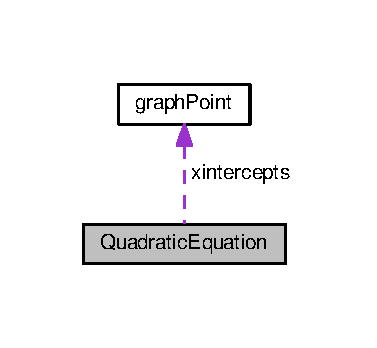
\includegraphics[width=181pt]{classQuadraticEquation__coll__graph}
\end{center}
\end{figure}
\subsection*{Public Member Functions}
\begin{DoxyCompactItemize}
\item 
\hyperlink{classQuadraticEquation_a3d5ca7fc85ff97aa3bd58f8c34e086b8}{Quadratic\+Equation} (double A=0.\+0, double B=0.\+0, double C=0.\+0)
\item 
\hyperlink{classQuadraticEquation_a16dcf4de9fb30312e2d5b19c9e30eb00}{$\sim$\+Quadratic\+Equation} ()
\item 
int \hyperlink{classQuadraticEquation_afffee8be484997e6b7fb716cfcef1438}{getxintercepts} ()
\item 
void \hyperlink{classQuadraticEquation_a196dc91dd16021f0ba54cc4e2b36da12}{displayequation} ()
\end{DoxyCompactItemize}
\subsection*{Public Attributes}
\begin{DoxyCompactItemize}
\item 
double \hyperlink{classQuadraticEquation_ac75fc269faf1b22dbae9256a67823627}{a}
\item 
double \hyperlink{classQuadraticEquation_a7c3b8208e2d36d576d17bee5a7ce812f}{b}
\item 
double \hyperlink{classQuadraticEquation_a3ea57c6e9d39a8f4ee2b029db6a8e6d8}{c}
\item 
\hyperlink{structgraphPoint}{graph\+Point} \hyperlink{classQuadraticEquation_a5001f513b8982984dd1b2efe43972d37}{xintercepts} \mbox{[}2\mbox{]}
\end{DoxyCompactItemize}


\subsection{Constructor \& Destructor Documentation}
\index{Quadratic\+Equation@{Quadratic\+Equation}!Quadratic\+Equation@{Quadratic\+Equation}}
\index{Quadratic\+Equation@{Quadratic\+Equation}!Quadratic\+Equation@{Quadratic\+Equation}}
\subsubsection[{\texorpdfstring{Quadratic\+Equation(double A=0.\+0, double B=0.\+0, double C=0.\+0)}{QuadraticEquation(double A=0.0, double B=0.0, double C=0.0)}}]{\setlength{\rightskip}{0pt plus 5cm}Quadratic\+Equation\+::\+Quadratic\+Equation (
\begin{DoxyParamCaption}
\item[{double}]{A = {\ttfamily 0.0}, }
\item[{double}]{B = {\ttfamily 0.0}, }
\item[{double}]{C = {\ttfamily 0.0}}
\end{DoxyParamCaption}
)\hspace{0.3cm}{\ttfamily [inline]}}\hypertarget{classQuadraticEquation_a3d5ca7fc85ff97aa3bd58f8c34e086b8}{}\label{classQuadraticEquation_a3d5ca7fc85ff97aa3bd58f8c34e086b8}

\begin{DoxyCode}
11                                                                       : \hyperlink{classQuadraticEquation_ac75fc269faf1b22dbae9256a67823627}{a}(A), \hyperlink{classQuadraticEquation_a7c3b8208e2d36d576d17bee5a7ce812f}{b}(B), 
      \hyperlink{classQuadraticEquation_a3ea57c6e9d39a8f4ee2b029db6a8e6d8}{c}(C)\{
12         \hyperlink{classQuadraticEquation_a5001f513b8982984dd1b2efe43972d37}{xintercepts}[0].\hyperlink{structgraphPoint_a49dfdf1225bd73da89c1b454cdd1ae84}{x} = 0.0;
13         \hyperlink{classQuadraticEquation_a5001f513b8982984dd1b2efe43972d37}{xintercepts}[0].\hyperlink{structgraphPoint_a7b34c65aec2d9df8647e6215060cb9be}{y} = 0.0;
14         \hyperlink{classQuadraticEquation_a5001f513b8982984dd1b2efe43972d37}{xintercepts}[1].\hyperlink{structgraphPoint_a49dfdf1225bd73da89c1b454cdd1ae84}{x} = 0.0;
15         \hyperlink{classQuadraticEquation_a5001f513b8982984dd1b2efe43972d37}{xintercepts}[1].\hyperlink{structgraphPoint_a7b34c65aec2d9df8647e6215060cb9be}{y} = 0.0;
16     \}
\end{DoxyCode}
\index{Quadratic\+Equation@{Quadratic\+Equation}!````~Quadratic\+Equation@{$\sim$\+Quadratic\+Equation}}
\index{````~Quadratic\+Equation@{$\sim$\+Quadratic\+Equation}!Quadratic\+Equation@{Quadratic\+Equation}}
\subsubsection[{\texorpdfstring{$\sim$\+Quadratic\+Equation()}{~QuadraticEquation()}}]{\setlength{\rightskip}{0pt plus 5cm}Quadratic\+Equation\+::$\sim$\+Quadratic\+Equation (
\begin{DoxyParamCaption}
{}
\end{DoxyParamCaption}
)\hspace{0.3cm}{\ttfamily [inline]}}\hypertarget{classQuadraticEquation_a16dcf4de9fb30312e2d5b19c9e30eb00}{}\label{classQuadraticEquation_a16dcf4de9fb30312e2d5b19c9e30eb00}

\begin{DoxyCode}
17 \{\}
\end{DoxyCode}


\subsection{Member Function Documentation}
\index{Quadratic\+Equation@{Quadratic\+Equation}!displayequation@{displayequation}}
\index{displayequation@{displayequation}!Quadratic\+Equation@{Quadratic\+Equation}}
\subsubsection[{\texorpdfstring{displayequation()}{displayequation()}}]{\setlength{\rightskip}{0pt plus 5cm}void Quadratic\+Equation\+::displayequation (
\begin{DoxyParamCaption}
{}
\end{DoxyParamCaption}
)\hspace{0.3cm}{\ttfamily [inline]}}\hypertarget{classQuadraticEquation_a196dc91dd16021f0ba54cc4e2b36da12}{}\label{classQuadraticEquation_a196dc91dd16021f0ba54cc4e2b36da12}

\begin{DoxyCode}
40                           \{
41         \textcolor{keywordflow}{if}(\hyperlink{classQuadraticEquation_ac75fc269faf1b22dbae9256a67823627}{a} != 0)\{
42             cout << \hyperlink{classQuadraticEquation_ac75fc269faf1b22dbae9256a67823627}{a};
43             cout << \textcolor{stringliteral}{"x^2"};\}
44         \textcolor{keywordflow}{if}(\hyperlink{classQuadraticEquation_a7c3b8208e2d36d576d17bee5a7ce812f}{b} >= 1 & \hyperlink{classQuadraticEquation_ac75fc269faf1b22dbae9256a67823627}{a} != 0)
45             cout << \textcolor{stringliteral}{"+"};
46         \textcolor{keywordflow}{if}(\hyperlink{classQuadraticEquation_a7c3b8208e2d36d576d17bee5a7ce812f}{b} != 0)
47             cout << \hyperlink{classQuadraticEquation_a7c3b8208e2d36d576d17bee5a7ce812f}{b} << \textcolor{stringliteral}{"x"};
48         \textcolor{keywordflow}{if}(\hyperlink{classQuadraticEquation_a3ea57c6e9d39a8f4ee2b029db6a8e6d8}{c} > 0)
49             cout << \textcolor{stringliteral}{"+"};
50         \textcolor{keywordflow}{if}(\hyperlink{classQuadraticEquation_a3ea57c6e9d39a8f4ee2b029db6a8e6d8}{c} != 0)
51             cout << \hyperlink{classQuadraticEquation_a3ea57c6e9d39a8f4ee2b029db6a8e6d8}{c};
52         \textcolor{keywordflow}{if}(\hyperlink{classQuadraticEquation_ac75fc269faf1b22dbae9256a67823627}{a} == 0 & b == 0 & c == 0)
53             cout << 0;
54         cout << \textcolor{stringliteral}{"=0"} << endl;
55     \}
\end{DoxyCode}
\index{Quadratic\+Equation@{Quadratic\+Equation}!getxintercepts@{getxintercepts}}
\index{getxintercepts@{getxintercepts}!Quadratic\+Equation@{Quadratic\+Equation}}
\subsubsection[{\texorpdfstring{getxintercepts()}{getxintercepts()}}]{\setlength{\rightskip}{0pt plus 5cm}int Quadratic\+Equation\+::getxintercepts (
\begin{DoxyParamCaption}
{}
\end{DoxyParamCaption}
)\hspace{0.3cm}{\ttfamily [inline]}}\hypertarget{classQuadraticEquation_afffee8be484997e6b7fb716cfcef1438}{}\label{classQuadraticEquation_afffee8be484997e6b7fb716cfcef1438}

\begin{DoxyCode}
20                         \{
21 
22 
23         \textcolor{keywordtype}{double} temp = (\hyperlink{classQuadraticEquation_a7c3b8208e2d36d576d17bee5a7ce812f}{b} * \hyperlink{classQuadraticEquation_a7c3b8208e2d36d576d17bee5a7ce812f}{b}) - (4 * \hyperlink{classQuadraticEquation_ac75fc269faf1b22dbae9256a67823627}{a} * \hyperlink{classQuadraticEquation_a3ea57c6e9d39a8f4ee2b029db6a8e6d8}{c});
24         \textcolor{keywordflow}{if}(temp < 0)\{
25             cout << \textcolor{stringliteral}{"##-Square Root Error:\(\backslash\)n"}
26                  << \textcolor{stringliteral}{" ##- SquareRoot ( "} << temp << \textcolor{stringliteral}{" )\(\backslash\)n"};
27             \textcolor{keywordflow}{return} 1;
28         \}
29 
30         temp = sqrt ( temp );
31 
32         \hyperlink{classQuadraticEquation_a5001f513b8982984dd1b2efe43972d37}{xintercepts}[0].\hyperlink{structgraphPoint_a49dfdf1225bd73da89c1b454cdd1ae84}{x} = (\hyperlink{classQuadraticEquation_a7c3b8208e2d36d576d17bee5a7ce812f}{b} * -1) - temp;
33         \hyperlink{classQuadraticEquation_a5001f513b8982984dd1b2efe43972d37}{xintercepts}[0].\hyperlink{structgraphPoint_a49dfdf1225bd73da89c1b454cdd1ae84}{x} = \hyperlink{classQuadraticEquation_a5001f513b8982984dd1b2efe43972d37}{xintercepts}[0].\hyperlink{structgraphPoint_a49dfdf1225bd73da89c1b454cdd1ae84}{x} / (2 * \hyperlink{classQuadraticEquation_ac75fc269faf1b22dbae9256a67823627}{a});
34 
35         \hyperlink{classQuadraticEquation_a5001f513b8982984dd1b2efe43972d37}{xintercepts}[1].\hyperlink{structgraphPoint_a49dfdf1225bd73da89c1b454cdd1ae84}{x}  = (\hyperlink{classQuadraticEquation_a7c3b8208e2d36d576d17bee5a7ce812f}{b} * -1) + temp;
36         \hyperlink{classQuadraticEquation_a5001f513b8982984dd1b2efe43972d37}{xintercepts}[1].\hyperlink{structgraphPoint_a49dfdf1225bd73da89c1b454cdd1ae84}{x} = \hyperlink{classQuadraticEquation_a5001f513b8982984dd1b2efe43972d37}{xintercepts}[1].\hyperlink{structgraphPoint_a49dfdf1225bd73da89c1b454cdd1ae84}{x} / (2 * \hyperlink{classQuadraticEquation_ac75fc269faf1b22dbae9256a67823627}{a});
37         \textcolor{keywordflow}{return} 0;
38     \}
\end{DoxyCode}


\subsection{Member Data Documentation}
\index{Quadratic\+Equation@{Quadratic\+Equation}!a@{a}}
\index{a@{a}!Quadratic\+Equation@{Quadratic\+Equation}}
\subsubsection[{\texorpdfstring{a}{a}}]{\setlength{\rightskip}{0pt plus 5cm}double Quadratic\+Equation\+::a}\hypertarget{classQuadraticEquation_ac75fc269faf1b22dbae9256a67823627}{}\label{classQuadraticEquation_ac75fc269faf1b22dbae9256a67823627}
\index{Quadratic\+Equation@{Quadratic\+Equation}!b@{b}}
\index{b@{b}!Quadratic\+Equation@{Quadratic\+Equation}}
\subsubsection[{\texorpdfstring{b}{b}}]{\setlength{\rightskip}{0pt plus 5cm}double Quadratic\+Equation\+::b}\hypertarget{classQuadraticEquation_a7c3b8208e2d36d576d17bee5a7ce812f}{}\label{classQuadraticEquation_a7c3b8208e2d36d576d17bee5a7ce812f}
\index{Quadratic\+Equation@{Quadratic\+Equation}!c@{c}}
\index{c@{c}!Quadratic\+Equation@{Quadratic\+Equation}}
\subsubsection[{\texorpdfstring{c}{c}}]{\setlength{\rightskip}{0pt plus 5cm}double Quadratic\+Equation\+::c}\hypertarget{classQuadraticEquation_a3ea57c6e9d39a8f4ee2b029db6a8e6d8}{}\label{classQuadraticEquation_a3ea57c6e9d39a8f4ee2b029db6a8e6d8}
\index{Quadratic\+Equation@{Quadratic\+Equation}!xintercepts@{xintercepts}}
\index{xintercepts@{xintercepts}!Quadratic\+Equation@{Quadratic\+Equation}}
\subsubsection[{\texorpdfstring{xintercepts}{xintercepts}}]{\setlength{\rightskip}{0pt plus 5cm}{\bf graph\+Point} Quadratic\+Equation\+::xintercepts\mbox{[}2\mbox{]}}\hypertarget{classQuadraticEquation_a5001f513b8982984dd1b2efe43972d37}{}\label{classQuadraticEquation_a5001f513b8982984dd1b2efe43972d37}


The documentation for this class was generated from the following file\+:\begin{DoxyCompactItemize}
\item 
\hyperlink{QuadraticFormula_8cpp}{Quadratic\+Formula.\+cpp}\end{DoxyCompactItemize}

\chapter{File Documentation}
\hypertarget{QuadraticFormula_8cpp}{}\section{Quadratic\+Formula.\+cpp File Reference}
\label{QuadraticFormula_8cpp}\index{Quadratic\+Formula.\+cpp@{Quadratic\+Formula.\+cpp}}
{\ttfamily \#include $<$math.\+h$>$}\\*
{\ttfamily \#include $<$iostream$>$}\\*
Include dependency graph for Quadratic\+Formula.\+cpp\+:
\nopagebreak
\begin{figure}[H]
\begin{center}
\leavevmode
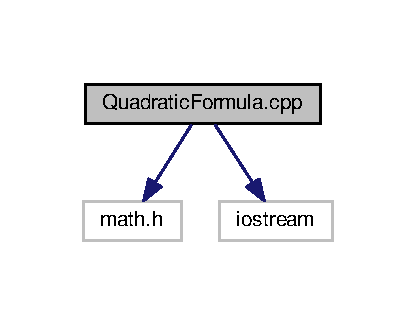
\includegraphics[width=200pt]{QuadraticFormula_8cpp__incl}
\end{center}
\end{figure}
\subsection*{Classes}
\begin{DoxyCompactItemize}
\item 
struct \hyperlink{structgraphPoint}{graph\+Point}
\item 
class \hyperlink{classQuadraticEquation}{Quadratic\+Equation}
\end{DoxyCompactItemize}
\subsection*{Functions}
\begin{DoxyCompactItemize}
\item 
void \hyperlink{QuadraticFormula_8cpp_ac55e9139cee9855d8999e57667a31a5b}{credits\+Help} ()
\item 
void \hyperlink{QuadraticFormula_8cpp_ae892baee905129ad78df12e61b99223a}{wierd\+Getch} ()
\item 
int \hyperlink{QuadraticFormula_8cpp_a0ddf1224851353fc92bfbff6f499fa97}{main} (int argc, char $\ast$argv\mbox{[}$\,$\mbox{]})
\end{DoxyCompactItemize}


\subsection{Function Documentation}
\index{Quadratic\+Formula.\+cpp@{Quadratic\+Formula.\+cpp}!credits\+Help@{credits\+Help}}
\index{credits\+Help@{credits\+Help}!Quadratic\+Formula.\+cpp@{Quadratic\+Formula.\+cpp}}
\subsubsection[{\texorpdfstring{credits\+Help()}{creditsHelp()}}]{\setlength{\rightskip}{0pt plus 5cm}void credits\+Help (
\begin{DoxyParamCaption}
{}
\end{DoxyParamCaption}
)}\hypertarget{QuadraticFormula_8cpp_ac55e9139cee9855d8999e57667a31a5b}{}\label{QuadraticFormula_8cpp_ac55e9139cee9855d8999e57667a31a5b}

\begin{DoxyCode}
115                   \{
116 
117     cout << \textcolor{stringliteral}{"\(\backslash\)nThis program was created by me to make my math homework easier\(\backslash\)n\(\backslash\)n"}
118 
119          << \textcolor{stringliteral}{"What it does:\(\backslash\)n"}
120          << \textcolor{stringliteral}{"It takes in the 'a', 'b', and 'c' values for a quadratic equation\(\backslash\)n"}
121          << \textcolor{stringliteral}{"which equals zero.\(\backslash\)n"}
122          << \textcolor{stringliteral}{"EX: \(\backslash\)"x^2 - 3x + 2 = 0\(\backslash\)" is equal to \(\backslash\)"(x - 2)(x - 1) = 0\(\backslash\)"\(\backslash\)n"}
123          << \textcolor{stringliteral}{"    ax^2 + bx + c = 0\(\backslash\)n"}
124          << \textcolor{stringliteral}{"    The 'a','b', and 'c' values for the equation would be 1, -3, and 2\(\backslash\)n"}
125          << \textcolor{stringliteral}{"    The x intercepts for this would be (2, 0) and (1, 0)\(\backslash\)n"}
126          << \textcolor{stringliteral}{"    2^2 - 3(2) + 2 = 0 and 1^2 - 3(1) + 2 = 0\(\backslash\)n\(\backslash\)n"}
127 
128          << \textcolor{stringliteral}{"Why would I use this:\(\backslash\)n"}
129          << \textcolor{stringliteral}{"1) You are in Algebra I/II or Geometry\(\backslash\)n"}
130          << \textcolor{stringliteral}{"2) Your too lazy to do the quadratic equation on your own which is:\(\backslash\)n"}
131          << \textcolor{stringliteral}{"   x=( -b +/- sqrt(bb - 4ac) ) / (2a)\(\backslash\)n"};
132     \hyperlink{QuadraticFormula_8cpp_ae892baee905129ad78df12e61b99223a}{wierdGetch}();
133     exit(0);
134 \}
\end{DoxyCode}


Here is the call graph for this function\+:
\nopagebreak
\begin{figure}[H]
\begin{center}
\leavevmode
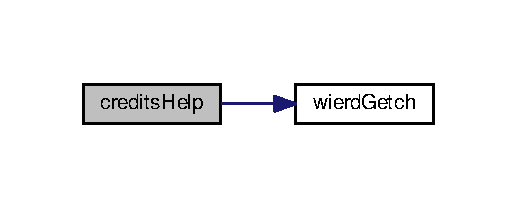
\includegraphics[width=248pt]{QuadraticFormula_8cpp_ac55e9139cee9855d8999e57667a31a5b_cgraph}
\end{center}
\end{figure}


\index{Quadratic\+Formula.\+cpp@{Quadratic\+Formula.\+cpp}!main@{main}}
\index{main@{main}!Quadratic\+Formula.\+cpp@{Quadratic\+Formula.\+cpp}}
\subsubsection[{\texorpdfstring{main(int argc, char $\ast$argv[])}{main(int argc, char *argv[])}}]{\setlength{\rightskip}{0pt plus 5cm}int main (
\begin{DoxyParamCaption}
\item[{int}]{argc, }
\item[{char $\ast$}]{argv\mbox{[}$\,$\mbox{]}}
\end{DoxyParamCaption}
)}\hypertarget{QuadraticFormula_8cpp_a0ddf1224851353fc92bfbff6f499fa97}{}\label{QuadraticFormula_8cpp_a0ddf1224851353fc92bfbff6f499fa97}

\begin{DoxyCode}
72                                 \{
73     cout << \textcolor{stringliteral}{"@-Quadratic Equation Solver\(\backslash\)n"}
74          << \textcolor{stringliteral}{" @-Karlan Mitchell karlanmitchell-at-comcast-dot-net\(\backslash\)n"}
75          << \textcolor{stringliteral}{" @-For Credits/Help enter 0 for A\(\backslash\)n"};
76 
77     \textcolor{keywordtype}{double} a,b,c;
78 
79     cout << \textcolor{stringliteral}{"Enter in values for equation\(\backslash\)n"};
80     \textcolor{keywordflow}{for}(;;)\{
81         cout << \textcolor{stringliteral}{"A: "};
82         cin >> a;
83         \textcolor{keywordflow}{if}(a == 0.0)\{
84             \hyperlink{QuadraticFormula_8cpp_ac55e9139cee9855d8999e57667a31a5b}{creditsHelp}();
85             \textcolor{keywordflow}{continue};
86         \}
87         \textcolor{keywordflow}{break};
88     \}
89     cout << \textcolor{stringliteral}{"B: "};
90     cin >> b;
91     cout << \textcolor{stringliteral}{"C: "};
92     cin >> c;
93 
94     \hyperlink{classQuadraticEquation}{QuadraticEquation} test(a,b,c);\textcolor{comment}{//create the class}
95 
96     test.displayequation();\textcolor{comment}{//display the equation with the class function}
97 
98     \textcolor{keywordflow}{switch}(test.getxintercepts())\{\textcolor{comment}{/* I am using a switch here instead of}
99 \textcolor{comment}{                               * an if because I constanly add/remove}
100 \textcolor{comment}{                   * error messages to this function*/}
101         \textcolor{keywordflow}{case} 1:
102             cout << \textcolor{stringliteral}{"!!-Equation not possible\(\backslash\)n"}
103                 << \textcolor{stringliteral}{" !!-If you know that it is possible, please contact me about a bug\(\backslash\)n"};
104             exit(1);
105             \textcolor{keywordflow}{break};
106     \}
107 
108     cout << \textcolor{stringliteral}{"x = "} << test.xintercepts[0].x << \textcolor{stringliteral}{" | "} << test.xintercepts[1].x << endl;
109     cout << \textcolor{stringliteral}{"("} << test.xintercepts[0].x << \textcolor{stringliteral}{", 0) & ("} << test.xintercepts[1].x << \textcolor{stringliteral}{", 0)\(\backslash\)n"};
110 
111 
112     \hyperlink{QuadraticFormula_8cpp_ae892baee905129ad78df12e61b99223a}{wierdGetch}();
113     \textcolor{keywordflow}{return} 0;
114 \}
\end{DoxyCode}


Here is the call graph for this function\+:
\nopagebreak
\begin{figure}[H]
\begin{center}
\leavevmode
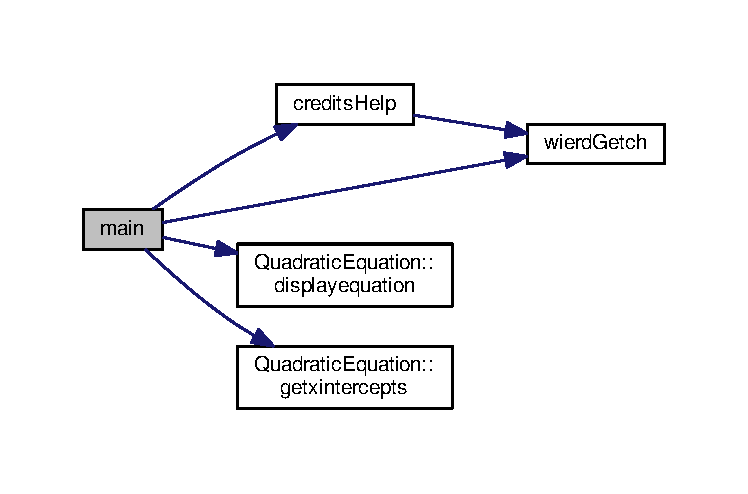
\includegraphics[width=350pt]{QuadraticFormula_8cpp_a0ddf1224851353fc92bfbff6f499fa97_cgraph}
\end{center}
\end{figure}


\index{Quadratic\+Formula.\+cpp@{Quadratic\+Formula.\+cpp}!wierd\+Getch@{wierd\+Getch}}
\index{wierd\+Getch@{wierd\+Getch}!Quadratic\+Formula.\+cpp@{Quadratic\+Formula.\+cpp}}
\subsubsection[{\texorpdfstring{wierd\+Getch()}{wierdGetch()}}]{\setlength{\rightskip}{0pt plus 5cm}void wierd\+Getch (
\begin{DoxyParamCaption}
{}
\end{DoxyParamCaption}
)}\hypertarget{QuadraticFormula_8cpp_ae892baee905129ad78df12e61b99223a}{}\label{QuadraticFormula_8cpp_ae892baee905129ad78df12e61b99223a}

\begin{DoxyCode}
135                  \{
136     cout << \textcolor{stringliteral}{"Press enter to exit..."};
137     getchar();getchar();\textcolor{comment}{//Why do I need, two?  The world may never know}
138 \}\end{DoxyCode}

%--- End generated contents ---

% Index
\backmatter
\newpage
\phantomsection
\clearemptydoublepage
\addcontentsline{toc}{chapter}{Index}
\printindex

\end{document}
